\section{Arquitectura de la Solución}

La figura X muestra un diagrama de arquitectura de la solución, para
soportar los procesos de análisis y extracción de datos, así como la
visualización de los mismos.
La participación de cada uno de los componentes de la solución en las distintas
etapas, será explicado en las próximas secciones.

\begin{figure}[H]
  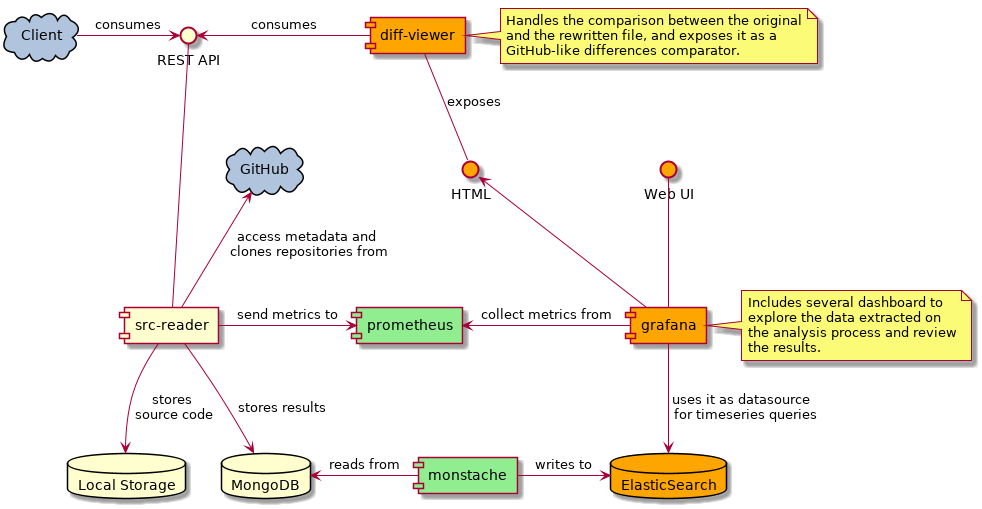
\includegraphics[width=12cm]{implementation/architecture_overview.png}
  \centering
  \caption{Arquitectura general de la Solución}
\end{figure}

\subsection{Fase: Cálculo}

Tal como se enunció anteriormente, la fase de cálculo consta de diferentes etapas,
cada una con un objetivo bien claro.
Estas etapas se suceden unas a otras, utilizando la salida de una estapa previamente
ejecutada, como entrada para la siguiente, presentando así una cierta secuencialidad.

%extracción, procesamiento y cálculo.

\subsubsection{Etapa: Extracción}

Para poder dividir y expandir los identificadores que forman parte de una base de código de fuente, 
primero necesitamos analizar los archivos que lo componen y construir los árboles de sintáxisis
abstracta, que serán procesados en la etapa siguiente.
Los pasos que forman parte 
Este proceso, definido como \textbf{extracción}, y contiene diferentes pasos,
dentro de los que encontramos:

\begin{enumerate}
  \item Clonación de repositorios de código.
  \item Filtrado de archivos.
  \item Construcción de ASTs.
\end{enumerate}

La etapa de extracción inicia con la \textbf{clonación del repositorio} elegido para ser
analizado. En el caso de nuestra solución, se requiere que el código fuente esté
versionado a través de la herramienta de control de versiones (TODO: SVCs, link) de \textit{git},
y disponible públicamente en la plataforma de \textit{GitHub} (TODO: link).
A través de las librerías correspondientes, el código es copiado a un directorio temporal,
para luego ser procesado.

Como no todos los archivos que forman parte de un repositorio son de interés para la construcción
de un árbol de sintáxis abstracta, aquellos que no formen parte del conjunto candidato, son
\textbf{filtrados}.
Esto implica que sólo los archivos de extensión \textit{.go} son considerados, exceptuando
los que tienen el sufijo \textit{\_test.go}, ya que contienen el código para las pruebas
unitarias y/o de integración, y por el momento se decidió descartar.

Por último, con el conjunto de archivos a analizar ya determinado, se procede a la
\textbf{construcción de los árboles de sintáxis abstracta}.
Para ello, el proceso se apoya en las librerías provistas dentro de la distribución
por defecto del lenguaje de programación, las cuales permiten leer los archivos,
hacer la \textit{tokenización} y \textit{parsing} de los mismos, con la consecuente
generación de los ASTs.

%TODO (incluir sección de AST y GO?)
%AST en Golang, convenciones de desarrollo, Effective Go, Levesthein distance.

Como resultado de esta etapa, tenemos un conjunto de ASTs, los cuales sirven como parámetros
de entrada para la etapa de procesamiento, la cual es explicada a continuación.

\subsubsection{Etapa: Procesamiento}

La correcta ejecución de algunos algoritmos, tanto de división como de expansión,
requiere cierta \textbf{información contextual}, extraída desde el código fuente.
Por ejemplo, y tal como se especificó en el capítulo X, el algorimo de división \textit{Samurai}
depende de dos tablas de frencuencias.
Una de estas tablas es específica al programa bajo análisis, mientras que la otra corresponde
a un universo mayor de código fuente, independiente del código en cuestión.
Así mismo, el algoritmo de \textit{Expansión Básica} utiliza listas tanto de palabras como frases,
extraídas de los comentarios e identificadores asociados a cada una de las funciones analizadas.
En el caso de \textit{AMAP}, para poder efectuar las expansiones, se necesitan establecer tablas
de frecuencia por métodos, clases, paquetes e incluso proyectos.

Esta información contextual necesaria, se extrae durante la etapa de \textbf{procesamiento},
al realizar un \textbf{análisis semántico} sobre los diferentes \textit{árboles de sintáxis abstracta (ASTs)} 
resultantes del paso anterior.

\subsubsection{Etapa: Cálculo}

Durante la etapa de \textbf{cálculo}, los identificadores son relevados desde el código fuente,
y los distintos algoritmos aplicados.
La aplicación de los algoritmos se hace de a pares, con una combinación preestablecida
entre división y expansión.

La expansión resultante, junto con el nombre original del identificador, son las
entradas para el cálculo de la métrica, aplicando la distancia de Levesthein
entre ambos.
De esta manera, se obtiene un valor que representa la distancia entre los mismos.

Cada identificador, junto con sus separaciones y expansiones obtenidas por los diferentes
algoritmos, y el valor de la métrica, son almacenadas en una base de datos.
De esta manera, luego es posible combinar los valores de cada, agregándolos al nivel
que se desee explorar (paquete o proyecto).

\subsection{Fase: Visualización}

Una vez completada la fase de cálculo, los resultados quedan disponibles para la
visualización de los mismos.
Para ello, hay dos componentes particulares.
Por un lado, el componente que permite la visualización de las métricas por proyecto,
a nivel general; y por otro, la herramienta que permite previsualizar un archivo
de código fuente, cambiando los nombres de los identificadores por su mejor expansión,
de acuerdo al valor de la métrica.

Las siguientes secciones explican al detalle los elementos de visualización, y
la forma correcta de interpretarlos.

\subsubsection{Visualización: Dashboard}



\subsubsection{Visualización: Rewrite}

La previsualización del reemplazo de los identificadores de un archivo
por el resultado del procesamiento de división, expansión y cálculo de distancia,
se realiza por medio de la herramienta \textsc{diff-viewer}.

Esta herramienta presenta una disposición similar al comparador de código
disponible en GitHub, donde se resalta tanto la línea de código como el texto modificado,
tal como puede verse en la figura X.

\begin{figure}[H]
  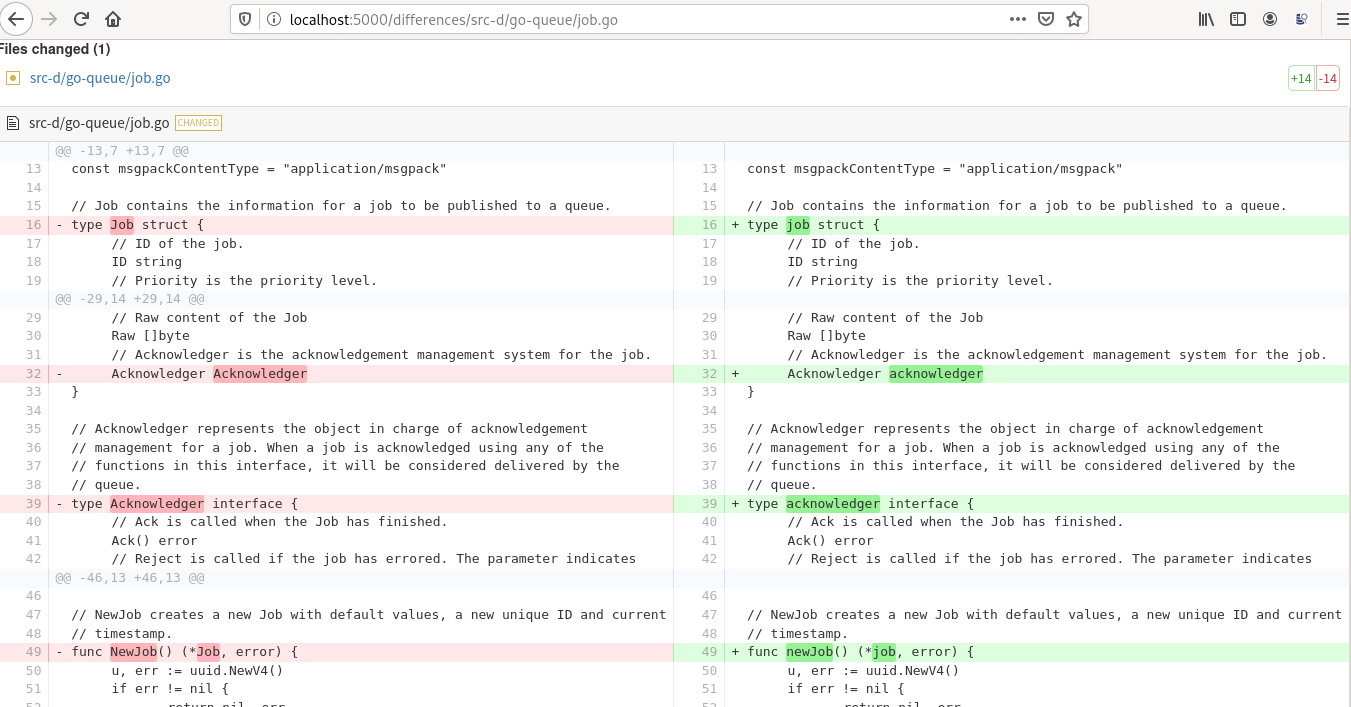
\includegraphics[width=12cm]{implementation/diff_viewer.png}
  \centering
  \caption{Previsualización de Diferencias}
\end{figure}

Esta herramienta particular, disponibiliza al usuario final, la siguiente
información:

\begin{itemize}
  \item Proyecto y archivo analizado.
  \item Cantidad total de modificaciones tentativas.
  \item Comparación línea por línea.
\end{itemize}

